\documentclass[12pt,a4paper]{mimosis}
\usepackage{newlfont}
\usepackage{amsmath}
\usepackage{epigraph}
\usepackage{amsfonts}
\usepackage{graphicx}
\usepackage{listings}
\usepackage{styles/bussproofs}

\usepackage[
  autocite     = plain,
  backend      = bibtex,
  doi          = true,
  url          = true,
  giveninits   = true,
  hyperref     = true,
  maxbibnames  = 99,
  maxcitenames = 2,
  sortcites    = false,
  style        = numeric,
  ]{biblatex}

% %%%%%%%%%%%%%%%%%%%%%%%%%%%%%%%%%%%%%%%%%%%%%%%%%%%%%%%%%%%%%%%%%%%%%%%%
% Some adjustments to make the bibliography more clean
%%%%%%%%%%%%%%%%%%%%%%%%%%%%%%%%%%%%%%%%%%%%%%%%%%%%%%%%%%%%%%%%%%%%%%%%
%
% The subsequent commands do the following:
%  - Removing the month field from the bibliography
%  - Fixing the Oxford commma
%  - Suppress the "in" for journal articles
%  - Remove the parentheses of the year in an article
%  - Delimit volume and issue of an article by a colon ":" instead of
%    a dot ""
%  - Use commas to separate the location of publishers from their name
%  - Remove the abbreviation for technical reports
%  - Display the label of bibliographic entries without brackets in the
%    bibliography
%  - Ensure that DOIs are followed by a non-breakable space
%  - Use hair spaces between initials of authors
%  - Make the font size of citations smaller
%  - Fixing ordinal numbers (1st, 2nd, 3rd, and so) on by using
%    superscripts

% Remove the month field from the bibliography. It does not serve a good
% purpose, I guess. And often, it cannot be used because the journals
% have some crazy issue policies.
\AtEveryBibitem{\clearfield{month}}
\AtEveryCitekey{\clearfield{month}}

% Fixing the Oxford comma. Not sure whether this is the proper solution.
% More information is available under [1] and [2].
%
% [1] http://tex.stackexchange.com/questions/97712/biblatex-apa-style-is-missing-a-comma-in-the-references-why
% [2] http://tex.stackexchange.com/questions/44048/use-et-al-in-biblatex-custom-style
%
\AtBeginBibliography{%
  \renewcommand*{\finalnamedelim}{%
    \ifthenelse{\value{listcount} > 2}{%
      \addcomma
      \addspace
      \bibstring{and}%
    }{%
      \addspace
      \bibstring{and}%
    }
  }
}

% Suppress "in" for journal articles. This is unnecessary in my opinion
% because the journal title is typeset in italics anyway.
\renewbibmacro{in:}{%
  \ifentrytype{article}
  {%
  }%
  % else
  {%
    \printtext{\bibstring{in}\intitlepunct}%
  }%
}

% Remove the parentheses for the year in an article. This removes a lot
% of undesired parentheses in the bibliography, thereby improving the
% readability. Moreover, it makes the look of the bibliography more
% consistent.
\renewbibmacro*{issue+date}{%
  \setunit{\addcomma\space}
    \iffieldundef{issue}
      {\usebibmacro{date}}
      {\printfield{issue}%
       \setunit*{\addspace}%
       \usebibmacro{date}}%
  \newunit}

% Delimit the volume and the number of an article by a colon instead of
% by a dot, which I consider to be more readable.
\renewbibmacro*{volume+number+eid}{%
  \printfield{volume}%
  \setunit*{\addcolon}%
  \printfield{number}%
  \setunit{\addcomma\space}%
  \printfield{eid}%
}

% Do not use a colon for the publisher location. Instead, connect
% publisher, location, and date via commas.
\renewbibmacro*{publisher+location+date}{%
  \printlist{publisher}%
  \setunit*{\addcomma\space}%
  \printlist{location}%
  \setunit*{\addcomma\space}%
  \usebibmacro{date}%
  \newunit%
}

% Ditto for other entry types.
\renewbibmacro*{organization+location+date}{%
  \printlist{location}%
  \setunit*{\addcomma\space}%
  \printlist{organization}%
  \setunit*{\addcomma\space}%
  \usebibmacro{date}%
  \newunit%
}

% Display the label of a bibliographic entry in bare style, without any
% brackets. I like this more than the default.
%
% Note that this is *really* the proper and official way of doing this.
\DeclareFieldFormat{labelnumberwidth}{#1\adddot}

% Ensure that DOIs are followed by a non-breakable space.
\DeclareFieldFormat{doi}{%
  \mkbibacro{DOI}\addcolon\addnbspace
    \ifhyperref
      {\href{http://dx.doi.org/#1}{\nolinkurl{#1}}}
      %
      {\nolinkurl{#1}}
}

% Use proper hair spaces between initials as suggested by Bringhurst and
% others.
\renewcommand*\bibinitdelim {\addnbthinspace}
\renewcommand*\bibnamedelima{\addnbthinspace}
\renewcommand*\bibnamedelimb{\addnbthinspace}
\renewcommand*\bibnamedelimi{\addnbthinspace}

% Make the font size of citations smaller. Depending on your selected
% font, you might not need this.
\usepackage{relsize}
\renewcommand*{\citesetup}{%
  \biburlsetup
  \relsize{-.5}%
}

\DeclareLanguageMapping{english}{english-mimosis}

% Make hyperlinks extend to the author name if `\textcite` is being used
% instead of another cite command.

\DeclareFieldFormat{citehyperref}{%
  % Need this to avoid nested links
  \DeclareFieldAlias{bibhyperref}{noformat}%
  \bibhyperref{#1}%
}

\DeclareFieldFormat{textcitehyperref}{%
  % Need this to avoid nested links
  \DeclareFieldAlias{bibhyperref}{noformat}%
  \bibhyperref{%
    #1%
    \ifbool{cbx:parens}
      {\bibcloseparen\global\boolfalse{cbx:parens}}
      {}%
    }%
}

\savebibmacro{cite}
\savebibmacro{textcite}

\renewbibmacro*{cite}{%
  \printtext[citehyperref]{%
    \restorebibmacro{cite}%
    \usebibmacro{cite}}%
}

\renewbibmacro*{textcite}{%
  \ifboolexpr{
    ( not test {\iffieldundef{prenote}} and
      test {\ifnumequal{\value{citecount}}{1}} )
    or
    ( not test {\iffieldundef{postnote}} and
      test {\ifnumequal{\value{citecount}}{\value{citetotal}}} )
  }%
  {\DeclareFieldAlias{textcitehyperref}{noformat}}
  {}%
  \printtext[textcitehyperref]{%
    \restorebibmacro{textcite}%
    \usebibmacro{textcite}}%
}

\addbibresource{tesi.bib}


\graphicspath{ {./pic/} }

\nocite{*}
\lstset{language=Caml}
\lstset{mathescape=true}
\lstset{morekeywords={include,inductive} }
\lstset{basicstyle=\footnotesize\ttfamily,breaklines=true}

\begin{document}
\begin{titlepage}
  \begin{center}
    {{
      \Large{\textsc{Alma Mater Studiorum $\cdot$ Universit\`a di Bologna}}
    }} \rule[0.1cm]{15.8cm}{0.1mm}
    \rule[0.5cm]{15.8cm}{0.6mm}
    {\small{\bf SCUOLA DI SCIENZE\\
    Corso di Laurea in Informatica}}
  \end{center}
  \vspace{15mm}
  \begin{center}
    {\LARGE{\bf Da Matita a Dedukti}}\\
    \vspace{3mm}
    {\LARGE{\bf e ritorno}}\\
  \end{center}
  \vspace{40mm}
  \par
  \noindent
  \begin{minipage}[t]{0.47\textwidth}
  {\large{\bf Relatore:\\
  Chiar.mo Prof.\\ 
  Claudio Sacerdoti Coen}}
  \end{minipage}
  \hfill
  \begin{minipage}[t]{0.47\textwidth}\raggedleft
  {\large{\bf Presentata da:\\
  Mattia Girolimetto}}
  \end{minipage}
  \vspace{20mm}
  \begin{center}
  {\large{\bf I Appello di Laurea\\%inserire il numero della sessione in cui ci si laurea
  Anno Accademico 2022-2023}}%inserire l'anno accademico a cui si è iscritti
  \end{center}
\end{titlepage}

\begin{titlepage}
	\thispagestyle{empty}
	\topmargin=6.5cm
	\raggedleft
	\large
	\em
	A Clarissa, per avermi cambiato\\
  ~ \\
	A Cristina e Teodoro, \\ per avermi dato questa opportunità
	\newpage
	\clearpage{\pagestyle{empty}\cleardoublepage}
\end{titlepage}


\begin{titlepage}
	\thispagestyle{empty}
	\topmargin=6.5cm
	\raggedleft
	\large
	\em
  \epigraph{
    
La logica, come il whisky, perde il suo effetto benefico se assunta in quantità
  eccessive.
    }
  {Lord Dunsany}
	\clearpage{\pagestyle{empty}\cleardoublepage}
\end{titlepage}


\begin{center}
  \textsc{Sommario}
\end{center}

Dedukti è un software che agisce da type checker per definizioni, enunciati e prove
codificati nel calcolo che implementa. Quest'ultimo è sufficientemente espressivo da poter
rappresentare anche altri calcoli. Questo rende Dedukti un framework logico con il 
quale è possibile sviluppare un sistema di codifica che converta nel suo linguaggio
le dimostrazioni scritte per altri proof assistant. 
Inizialmente si effettua un'analisi del processo di esportazione del codice da Matita
a Dedukti, Matita è un assistente alla dimostrazione sviluppato presso l'Università di
Bologna, basato sul calcolo delle costruzioni (co)-induttive. Successivamente si illustra 
la funzionalità di importazione del codice Dedukti in Matita e si esaminano le sfide che
si presentano nel ricostruire i termini originali di Matita, a partire dal codice Dedukti 
esportato in precedenza.


\thispagestyle{empty}
\tableofcontents

\chapter{Introduzione}
I \textit{proof assistant} sono software in grado di verificare una dimostrazione
formale scritta da un utente. Questa viene rappresentata internamente attraverso 
termini di un linguaggio funzionale dotato di un sistema di tipi avanzato, tale
da renderlo equivalente a una logica. Il loro sviluppo, negli anni, ha portato a una 
frammentazione della conoscenza in quanto sistemi diversi, che usano logiche diverse,
non sono compatibili tra loro. Per ovviare a questo problema un gruppo di ricercatori
dell'INRIA ha creato \textit{Dedukti}, la cui idea è quella di agire da \textit{type
checker} per definizioni, enunciati e prove codificati nel calcolo che implementa. 
Tale calcolo è sufficientemente espressivo per rappresentare in Dedukti qualunque
sistema di tipi, ovvero qualunque linguaggio funzionale con un sistema di tipi avanzato.
Questo rende Dedukti un \textit{logical framework}, ovvero un calcolo che svolge il 
ruolo di meta-calcolo per la rappresentazione uniforme di altri calcoli. Grazie a
esso è possibile sviluppare un sistema di codifica che converta dimostrazioni scritte
nel linguaggio di altri proof assistant, come \textit{Coq} e \textit{HOL lite}, nel
metalinguaggio di Dedukti. Proprio per questo all'INRIA è stato sviluppato \textit{Krajono},
un \textit{fork} di \textit{Matita}, che a sua volta è un proof assistant in sviluppo
nel Dipartimento di Informatica Scienze e Ingegneria dell'Università di Bologna.
Krajono permette di esportare le definizioni e i teoremi dati in Matita verso Dedukti,
attraverso una codifica del calcolo di Matita in quello di Dedukti. Krajono tuttavia 
non è più mantenuto e pertanto non integra le funzionalità del Matita \textit{baseline}
sviluppate negli ultimi anni. Il lavoro di questa tesi è diviso in due parti: la prima
prevede l'integrazione della funzionalità di esportazione di Krajono nel Matita odierno,
mentre l'obiettivo della seconda consiste nell'implementare la possibilità di reimportare
codice Dedukti esportato precedentemente da Matita. Il secondo punto in particolare 
ha richiesto la risoluzione di una serie di problemi, in primis dovuti al fatto che
il linguaggio di Matita sia più rigido e strutturato del metalinguaggio di Dedukti,
pertanto durante l'esportazione vengono perse informazioni necessarie alla
ricostruzione del codice originale. Ciò è stato risolto dotando l'export di
un meccanismo per preservarle dove necessario. In secondo luogo i sistemi di tipi
codificati in Dedukti, per essere consistenti, richiedono che le regole di riscrittura
scelte dagli sviluppatori per implementare la codifica siano confluenti e normalizzanti.
Dedukti non effettua questa verifica, che demanda a altri strumenti. Matita, invece, impone
un insieme molto restrittivo di controlli sintattici per garantire confluenza e terminazione,
che sono in generale proprietà indecidibili. Pertanto, quando si inverte il processo di
esportazione, sorge la necessità di ricostruire termini che soddisfino le condizioni 
sintattiche di Matita, che sono sufficienti, ma non necessarie, e che potrebbero essere
state violate durante la codifica in Dedukti, nonostante le regole fossero anche confluenti
e normalizzanti.

\chapter{Prerequisiti}
In questo capitolo vengono trattati prerequisiti necessari per la
comprensione del lavoro esposto nei capitoli quelli successivi. Nella sezione \ref{teoriaDeiTipi}
sono illustrati i fondamenti della \textit{Teoria dei Tipi}, teoria alla base 
di questa tesi. Nella sezione \ref{proofAssistant} vengono presentati Matita e Dedukti,
i software protagonisti di questo lavoro.

\section{La teoria dei tipi} \label{teoriaDeiTipi}
\subsection{La teoria dei tipi}
La \textit{teoria dei tipi} è una branca della logica e dell'informatica teorica il
cui obiettivo è quello di studiare i cosiddetti \textit{type system}, ovvero
insiemi di regole che associano una proprietà chiamata \textit{tipo} a degli oggetti
chiamati \textit{termini}. Intuitivamente, assegnare un tipo a un termine significa
assegnare al termine un'etichetta che rappresenta la natura del termine stesso.
Esempi comuni possono essere: 
\begin{itemize}
  \item $42$ è un numero naturale 
  \item $-5$ è un numero intero
  \item $falso$ è un valore di verità 
\end{itemize}

Formalmente si usa rappresentare queste espressioni separando il termine dal tipo usando
il simbolo ``$:$''. 

In teoria dei tipi, anche le funzioni sono termini e possono essere
a loro volta tipizzate. Ad esempio, la seguente funzione rappresentata attraverso un $\lambda$-termine
del $\lambda$-calcolo di Church 
\begin{center}
  $(\lambda$ $x$ $:$ $\mathbb{N}$ $.$ $x + x)$
\end{center}

è definita dall'insieme $\mathbb{N}$ a $\mathbb{N}$ stesso, e pertanto si dice che ha tipo $\mathbb{N} \rightarrow \mathbb{N}$

\subsection{L'isomorfismo di Curry-Howard}
Durante il '900 i logici Haskell Curry e William Alvin Howard, scoprirono una
corrispondenza diretta tra prove formali e programmi. In particolare notarono
che gli operatori logici e le regole usate durante una dimostrazione formale
sono equivalenti a tipi e costrutti usati nei programmi scritti usando linguaggi
di programmazione funzionali. Ne segue che il verificare la correttezza di una
prova corrisponde al verificare la correttezza degli assegnamenti di tipo di un
programma. Nella sua formulazione più generale, l'isomorfismo di Curry-Howard
può essere riassunto con la seguente tabella:

\begin{center}
  \begin{tabular}{ | c | c |}
    \hline
    \textbf{Operatori logici} & \textbf{Tipi} \\
    \hline
    $\top$ & Tipo unit \\
    \hline
    $\bot $ & Tipo vuoto/void \\
    \hline
   $\wedge$ & Tipi prodotto \\  
    \hline
   $\vee$ & Tipi somma \\
    \hline
   $\Rightarrow$ & Tipi funzione \\ 
    \hline
   $\exists$ & Tipi $\Sigma$ \\ 
    \hline
    $\forall $ & Tipi $\Pi$ \\ 
    \hline

  \end{tabular}
\end{center}

\subsection{La teoria dei tipi nella pratica}
La teoria dei tipi trova quindi grande applicazione nel campo dell'informatica
grazie allo studio e allo sviluppo dei linguaggi di programmazione. Inoltre,
ha permesso lo sviluppo di dimostratori interattivi di teoremi grazie all'
isomorfismo di Curry-Howard.

\section{Dedukti e Matita}\label{proofAssistant}
\subsection{Dimostratori interattivi di teoremi} 
Un dimostratore interattivo di teoremi (o \textit{proof assistant}) è un software 
che permette all'utente di costruire e verificare delle dimostrazioni matematiche
formali. Presa in input una prova espressa utilizzando uno specifico linguaggio 
formale il software è in grado di
verificarne la correttezza. In questo modo si possono costruire dimostrazioni
in modo interattivo, controllando progressivamente la correttezza di ogni passo.
Uno dei benefici chiave dell'usare un dimostratore interattivo automatico è l'abilità
di eliminare gli errori e le ambiguità che possono comparire nelle 
dimostrazioni tradizionali.

Durante la fase di verifica, il proof assistant rappresenta 
i termini della dimostrazione utilizzando un linguaggio di programmazione dotato di
un sistema di tipi avanzato, ottenendo alla fine una rappresentazione che può essere
considerata equivalente a un programma. Successivamente esegue un processo di \textit{
  type checking} in cui verifica la correttezza degli assegnamenti di tipo del programma.
Grazie all'isomorfismo di Curry-Howard questo equivale a verificare la correttezza della 
prova.

Il numero di proof assistant è aumentato nel tempo. Ciò è sicuramente un segnale
positivo per la comunità scientifica, in quanto dimostra un crescente interesse
verso lo sviluppo di questi strumenti. Tuttavia, questo aumento, unito al fatto
che proof assistant diversi sfruttano logiche diverse, porta a una frammentazione
della conoscenza. Per un utente non è quasi mai possibile, infatti, dimostrare la
veridicità di un teorema usando un proof assistant e usare la stessa dimostrazione
in un altro di questi tool senza doverla riscrivere.
Questo perché diversi proof assistant usano diversi sistemi di tipi e una dimostrazione,
per poter essere verificata con sistema di tipi diverso, deve essere tradotta.
Nasce dunque l'esigenza di favorire l'interoperabilità tra questi sistemi, in
modo da arginare questo problema e favorire lo sviluppo scientifico. 

\subsection{Dedukti}
Dedukti\footnote{``Dedurre'' in Esperanto} è un \textit{logical framework}, ovvero
un meta-sistema che consente di definire logiche e teoremi usando tali logiche.
È sviluppato da alcuni ricercatori del \textit{Institut National de Recherche
en Informatique et en Automatique} francese. Il software è open source, scritto
nel linguaggio di programmazione OCaml e distribuito secondo i termini della
CeCILL-B License. Uno degli obiettivi principali di Dedukti è creare
una connessione tra i diversi sistemi di dimostrazione assistita. Ciò significa
che le dimostrazioni possono essere tradotte da un sistema all'altro, agevolandone
lo scambio e il riutilizzo tra ambienti di lavoro diversi.
Infatti alcuni proof assistant, come ad esempio Coq e HOL Lite \footnote{Coq: https://github.com/Deducteam/CoqInE,\\ HOL Lite: https://arxiv.org/pdf/1507.08720.pdf},
godono già della possibilità di esportare e importare codice da e verso
Dedukti.
\begin{center}
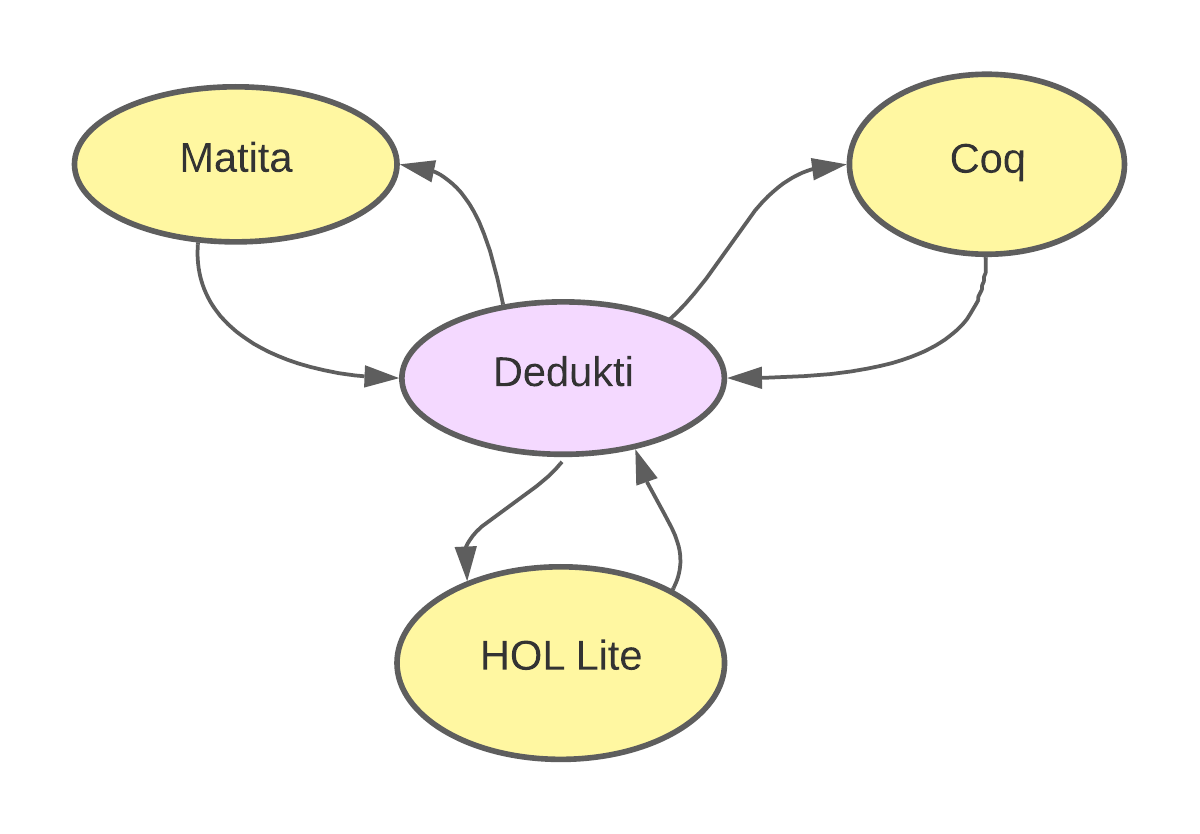
\includegraphics[scale=0.20]{schema1.png}
\end{center}

\paragraph{$\lambda\Pi$-Calcolo modulo}
Alla base di questo logical framework c'è il $\lambda\Pi$-calcolo modulo (o
semplicemente $\lambda\Pi$ modulo), un'estensione del $\lambda$-calcolo che introduce la \textit{tipizzazione dipendente} e le \textit{regole
di riscrittura}. La prima consente la specifica di tipi complessi che dipendono
dai valori delle espressioni, mentre le seconde consentono la trasformazione di
un'espressione in un'altra, seguendo determinate sostituzioni o manipolazioni.
La sintassi del $\lambda\Pi$ modulo è la seguente
\begin{center}
  \textit{Termini } \hspace{1pt} A, B, t, u \hspace{1pt} $::=$ Kind $\vert$ Type $\vert$ $\Pi$ x : A . B $\vert$ $\lambda$ x : A . B $\vert$ A B $\vert$ x \\
  \textit{Contesto} \hspace{1pt} $\Gamma$ \hspace{1pt} $::=$ $\emptyset$ $\vert$ $\Gamma$, x : A $\vert$ $\Gamma$, t $\hookrightarrow$ u
\end{center}

Mentre il sistema di tipi è definito dalle seguenti regole:

\begin{prooftree}
\AxiomC{}
\RightLabel{\textbf{Contesto vuoto}}
\UnaryInfC{[ ] \textit{ben formato}}
\end{prooftree}

\begin{prooftree}
\AxiomC{$\Gamma \vdash$ A : Type}
  \RightLabel{\textbf{Dichiarazione (Type)} $x \notin \Gamma$ }
\UnaryInfC{$\Gamma, x:A$ \textit{ben formato}}
\end{prooftree}

\begin{prooftree}
\AxiomC{$\Gamma \vdash$ A : Kind}
  \RightLabel{\textbf{Dichiarazione (Kind)} $x \notin \Gamma$ }
\UnaryInfC{$\Gamma,x:A$ \textit{ben formato}}
\end{prooftree}

\begin{prooftree}
\AxiomC{$\Gamma \vdash$ t $\hookrightarrow$ u \textit{ben formato}}
\RightLabel{\textbf{Regola}}
  \UnaryInfC{$\Gamma$, t $\hookrightarrow$ u \textit{ben formato}}
\end{prooftree}

\begin{prooftree}
\AxiomC{$\Gamma$ \textit{ben formato}}
\RightLabel{\textbf{Sorta}}
\UnaryInfC{$\Gamma \vdash$ Type : Kind}
\end{prooftree}

\begin{prooftree}
\AxiomC{$\Gamma$ \textit{ben formato}}
\AxiomC{x : A $\in \Gamma$}
\RightLabel{\textbf{Variabile}}
\BinaryInfC{$\Gamma \vdash$ x : A}
\end{prooftree}

\begin{prooftree}
\AxiomC{$\Gamma \vdash$ A : Type}
\AxiomC{$\Gamma,$ x : A $\vdash$ B : Type}
  \RightLabel{\textbf{Prodotto (Type)}}
\BinaryInfC{$\Gamma \vdash \Pi$ x : A . B  : Type}
\end{prooftree}

\begin{prooftree}
\AxiomC{$\Gamma \vdash$ A : Type}
\AxiomC{$\Gamma,$ x : A $\vdash$ B : Kind}
  \RightLabel{\textbf{Prodotto (Kind)}}
\BinaryInfC{$\Gamma \vdash \Pi$ x : A . B  : Kind}
\end{prooftree}

\begin{prooftree}
\AxiomC{$\Gamma \vdash$ A : Type}
\AxiomC{$\Gamma,$ x : A $\vdash$ B : Type}
\AxiomC{$\Gamma,$ x : A $\vdash$ t : B}
  \RightLabel{\textbf{$\boldsymbol{\lambda}$-astrazione}}
\TrinaryInfC{$\Gamma \vdash \lambda$ x : A . t  : $\Pi$ x : A . B}
\end{prooftree}

\begin{prooftree}
\AxiomC{$\Gamma \vdash$ t : $\Pi$ x : A . B}
\AxiomC{$\Gamma \vdash$ u : A}
\RightLabel{\textbf{Applicazione}}
  \BinaryInfC{$\Gamma \vdash$ (t u) : B $[$u/x$]$}
\end{prooftree}


\begin{prooftree}
\AxiomC{$\Gamma \vdash$ A : s}
\AxiomC{$\Gamma \vdash$ x : A}
\AxiomC{A $\equiv_{\beta\Gamma}$ B}
\RightLabel{\textbf{Equivalenza}}
\TrinaryInfC{$\Gamma \vdash$ x : B}
\end{prooftree}

\paragraph{Regole di riscrittura} \label{sottosezioneDedukti}
Le regole di riscrittura definiscono come trasformare o riscrivere espressioni
o termini secondo determinate regole specificate. Sono utili, ad esempio, per
implementare il processo di $\beta$-riduzione, che rappresenta il passo di 
applicazione di una funzione nei calcoli lambda:
\begin{center}
  ($\lambda$ x : A . f x) y $\hookrightarrow$ f y
\end{center}
Tuttavia, l'introduzione delle regole di riscrittura nel calcolo $\lambda\Pi$ 
lo rende non \textit{consistente}. Questo perché non vengono garantite le proprietà
di \textit{confluenza} e \textit{normalizzazione}.

La proprietà di confluenza (o di Church-Rosser) afferma che se ci sono due riduzioni distinte o sequenze di riduzioni
che possono essere applicate allo stesso termine, allora esiste un termine che
è raggiungibile da entrambi i risultati, applicando sequenze (possibilmente vuote)
di riduzioni aggiuntive. In altri termini, se esiste $a$ tale che $a \hookrightarrow^*$
$b$ e $a \hookrightarrow^*c$ allora esiste $d$ tale che $b \hookrightarrow^*d$ e
$c \hookrightarrow^* d$.

La proprietà di normalizzazione invece afferma che ogni termine può essere 
ridotto a una forma normale in un numero finito di passi di riduzione. In altre
parole, non ci sono sequenze infinite di riduzioni per un termine specifico. 
Questa proprietà è fondamentale per garantire la decidibilità di un calcolo. 


\subsection{Matita}
Matita è un  proof assistant in sviluppo nel dipartimento di Informatica Scienze
e Ingegneria dell'Università di Bologna. È open source, scritto nel linguaggio di
programmazione OCaml ed è rilasciato secondo i termini della GNU General Public Licence.
È basato sul \textit{calcolo delle costruzioni (co)induttive} (CIC), una teoria di tipi
dipendenti che estende il \textit{calcolo delle costruzioni} sviluppato da
Thierry Coquand aggiungendo i tipi induttivi, ovvero tipi autoreferenziali.
Le regole di tipaggio del CIC per i tipi semplici sono quelle comuni dei linguaggi
di programmazione. Di seguito sono riportate quelle per le  $\lambda$-astrazioni
e le applicazioni 

\begin{prooftree}
  \AxiomC{$\Gamma$, x : A $\vdash$ M : B}
  \RightLabel{\textbf{$\boldsymbol{\lambda}$-astrazione}}
  \UnaryInfC{$\Gamma \vdash (\lambda $x : A . M) : A $\rightarrow$ B}
\end{prooftree}

\begin{prooftree}
  \AxiomC{$\Gamma \vdash$ f : A $\rightarrow$ B}
  \AxiomC{$\Gamma \vdash$ x : A}
  \RightLabel{\textbf{Applicazione}}
  \BinaryInfC{$\Gamma \vdash (f$ $x)$ : B}
\end{prooftree}


CIC è più ricco del $\lambda\Pi$ modulo usato da Dedukti in quanto in più consente di definire 
\textit{tipi induttivi}, \textit{punti fissi} e \textit{pattern matching}.


I tipi induttivi consentono la creazione di tipi complessi e autoreferenziali e possono
essere utilizzati per definire strutture matematiche illimitate come liste,
alberi o grafi. L'esempio seguente mostra come si possa definire una lista concatenata
di numeri naturali usando Matita. Una struttura di questo tipo può essere vista come
una lista vuota oppure una coppia formata da un numero naturale e un'altra lista 
concatenata:

\begin{lstlisting}[mathescape]
include "basics/pts.ma".

inductive list : Type[0] $\stackrel{\text{def}}{=}$
   E : list
 | C : nat $\rightarrow$ list $\rightarrow$ list.

\end{lstlisting}

I punti fissi sono utili per definire funzioni ricorsive e, con l'aggiunta del
pattern matching, permettono di definire funzioni ricorsive strutturali. Un esempio
concreto di ciò è l'implementazione di una funzione per calcolare la lunghezza
di una lista basata sul pattern matching per ragionare sulla struttura della 
lista stessa:

\begin{lstlisting}
let rec len l on l $\stackrel{\text{def}}{=}$
 match l with
 [ E $\Rightarrow$ 0
 | C hd tl $\Rightarrow$ 1 + len tl
 ].
\end{lstlisting}


\chapter{Da Matita a Dedukti} \label{capitoloExport}
In questo capitolo viene prima introdotto \textit{Krajono}, il fork di Matita
da cui proviene il codice responsabile dell'export da Matita verso Dedukti. 
Successivamente viene analizzato nel dettaglio tecnico e teorico, il funzionamento 
di questa esportazione. Infine ne vengono discusse problematiche e limitazioni.

\section{Krajono}
Un team di ricercatori del \textit{Institut national de recherche en informatique 
et en automatique} ha sviluppato Krajono \footnote{Significa "Matita" in Esperanto}
\footnote{https://github.com/Deducteam/Krajono}. Krajono ha la possibilità
di esportare definizioni e teoremi dati in Matita verso Dedukti. Per far ciò
sfrutta una codifica del calcolo di Matita nel metalinguaggio di Dedukti. 
Tuttavia questo fork non è più mantenuto da anni.

\subsection{Integrazione in Matita}
In prima battuta, questo progetto consiste nell'integrare le funzionalità di 
esportazione di Krajono nella versione base di Matita. Tali funzionalità sono
state ottenute copiando i singoli sorgenti responsabili dell'esportazione 
all'interno di Matita.

Integrare direttamente queste funzionalità tramite \textit{pull request} tra
i \textit{repository Git}, comporterebbe complicazioni. Questo
è principalmente dovuto al fatto che Krajono non è stato mantenuto da anni ed
è basato su un fork separato di Matita chiamato \textit{Matita with embedded
Elpi}\footnote{https://github.com/LPCIC/matita}. 


\section{L'export}
\subsection{Il processo di esportazione}\label{sottosezioneProcessoDiExport}
\textit{Matitac} è il compilatore da linea di comando di Matita, se lo si lancia
compila tutti i file con estensione \textit{.ma} presenti nella directory corrente. 
Oppure è possibile compilare un singolo file passando come argomento il suo
nome.

Krajono fornisce la possibilità di attivare la funzionalità di export specificando l'argomento \texttt{-extract\_dedukti} a Matitac,
sia lavorando con un unico file sia con un'intera directory. A processo concluso 
si potranno trovare, nella directory dei sorgenti, i file \textit{.dk} contenenti
il codice matita esportato.

Quando il flag menzionato è attivo, il motore di Matita avvia il processo di
esportazione chiamando una specifica funzione da uno dei moduli OCaml importati
da Krajono. Questi moduli compiono delle analisi del tipo e della struttura del
termine Matita, con lo scopo di capire come applicare l'encoding appropriato.
Una volta costruiti, i termini Dedukti risultanti dalla codifica vengono inseriti
in una tabella hash, che alla fine del processo verrà scritta sul file \textit{.dk}
di output.

È importante notare come il processo di esportazione non è sempre un encoding
\textit{uno a uno}, ma determinate tipologie di termini Matita vengono codificati
in più termini Dedukti.

\subsection{L'encoding}\label{sottosezioneEncoding}
La codifica è composta da una serie di definizioni ed è contenuta dentro 
un modulo Dedukti chiamato ``cic''. 
Comprendere il funzionamento di questo modulo è essenziale per eseguire l'operazione
di importazione descritta nella sezione \ref{sezioneInvertireExport}, quindi 
verranno esaminati i punti più importanti.

Il modulo inizia fornendo le definizioni necessarie per rappresentare i numeri
naturali e l'operazione di massimo tra due numeri:

\begin{lstlisting}
Nat : Type.

z : Nat.
s : Nat -> Nat.

def m : Nat -> Nat -> Nat.
[i] m i z --> i.
[j] m z j --> j.
[i, j] m (s i) (s j) --> s (m i j).
\end{lstlisting}

È interessante vedere all'opera le regole di riscrittura per definire la costante
\texttt{m}. 

In seguito si procede alla codifica degli universi. Innanzitutto viene definito
il tipo \texttt{Sort} per rappresentare le sorte e successivamente vengono definite
la sorta \texttt{prop} e una funzione per rappresentare i diversi universi.

\begin{lstlisting}
Sort : Type.

prop : Sort.
type : Nat -> Sort.
\end{lstlisting}

Il naturale che \texttt{type} richiede in input rappresenta il numero dell'universo.
Ad esempio, l'universo \texttt{Type[3]} viene codificato come
\begin{lstlisting}
  type (s (s (s z)))
\end{lstlisting}

Più avanti nel modulo si passa alla codifica dei tipi.
Viene fornita la definizione di \texttt{Univ}, che accetta una sorta e restituisce 
un \texttt{Type} che rappresenta \textit{il codice} della sorta.

\begin{lstlisting}
Univ : Sort -> Type.
\end{lstlisting}

In seguito, si procede alla definizione della codifica dei termini utilizzando 
la definizione di \texttt{Term}. Questa funzione accetta una sorta, la sua
codifica associata e restituisce il termine corrispondente.

\begin{lstlisting}
def Term : s : Sort -> a : Univ s -> Type.
\end{lstlisting}

Viene poi definita \texttt{univ} con lo scopo di ritornare l'universo di una
data sorta.
\begin{lstlisting}
univ : s : Sort -> Univ (succ s).
\end{lstlisting}

\section{I problemi dell'export}

\subsection{I problemi di Krajono}
Krajono presenta diverse problematiche, la principale delle quali è il fatto che non
è più mantenuto da anni. È basato su una versione molto datata di Matita, che non
solo manca delle funzionalità moderne, ma richiede anche versioni obsolete delle 
sue dipendenze. Ciò rende Krajono difficile da installare e far funzionare.

Un'altra problematica riguarda la modalità con cui l'utente avvia l'esportazione.
Come evidenziato nella sezione \ref{sottosezioneProcessoDiExport}, l'unico modo
per avviarla è tramite il compilatore da linea di comando di Matita.
Questa funzionalità non è integrata nell'interfaccia grafica di Matita, né supporta
tutte le funzionalità fornite da essa.

Inoltre Krajono non esegue l'\textit{escaping} delle \textit{keyword} di Dedukti,
quindi quando viene esportato un termine con una keyword di Dedukti come nome, si
ottiene del codice non funzionante. Matita risolve questo problema aggiungendo un controllo adeguato durante
l'esportazione e, nel caso venga rilevato un conflitto, genera un nuovo nome per il 
termine. In questo modo si evitano potenziali errori e conflitti durante l'esportazione 
dei termini.

Infine l'esportazione non tiene traccia delle dipendenze tra i vari moduli Dedukti 
processati. Di conseguenza i file esportati non hanno alcuna informazione che li
lega alle loro dipendenze obbligando l'utente a ricostruirle manualmente.

\subsection{Perdita di informazione}
\paragraph{Normalizzazione e confluenza}
Dal punto di vista teorico, le problematiche dell'esportazione possono essere attribuite
alla differenza tra il $\lambda\Pi$-calcolo modulo e il calcolo delle costruzioni (co)induttive,
 pertanto non sono risolvibili. In particolare, come evidenziato nella sezione 
\ref{sottosezioneDedukti}, il $\lambda\Pi$-calcolo modulo non possiede le proprietà di normalizzazione
e confluenza che, al contrario, sono garantite dal calcolo delle costruzioni (co)induttive.

\paragraph{Proof irrelevance}
La \textit{proof irrelevance}, è un concetto nella teoria dei tipi che afferma che la prova di una 
proposizione o di un tipo non dovrebbe influire sul modo in cui questi vengono utilizzati.
Ciò significa che due dimostrazioni diverse, di una stessa proposizione o tipo, possono essere
considerate equivalenti e scambiate tra loro senza influire sulle conclusioni. In altre parole,
una volta dimostrata una proprietà o un tipo, la specifica dimostrazione della sua validità 
diventa irrilevante. Grazie alla proof irrelevance si può semplificare l'utilizzo dei tipi e delle
proposizioni dimostrate, poiché non è necessario considerare le specifiche dimostrazioni ogni volta,
quando si ragiona su di essi. 

Durante l'esportazione, le informazioni sulla proof irrelevance dei vari termini Matita vengono 
completamente perse.

\paragraph{Costrutti di Matita}
Alcuni costrutti di Matita non hanno una traduzione diretta in Dedukti
e pertanto vengono codificati come un blocco di termini. Durante la codifica
perdono quindi la loro natura originale e con essa alcuni attributi chiave, 
senza i quali diventa impossibile ricostruire il termine di partenza. 
Questo rappresenta un problema che verrà affrontato nella sezione \ref{sezioneInvertireExport}. 

\chapter{Da Dedukti a Matita}
In questo capitolo viene illustrato il funzionamento del processo di importazione
del codice Dedukti in Matita. Prima viene discussa l'integrazione del parser 
di Dedukti, successivamente viene analizzata la strategia usata per la traduzione
dei termini da un sistema all'altro. Infine viene trattata la ricostruzione
di oggetti Matita precedentemente esportati.

\section{Dedukti in Matita}
Come visto nel capitolo \ref{capitoloExport}, Krajono consente l'esportazione del codice
Matita verso Dedukti, tuttavia non è possibile fare il contrario. L'export è dunque 
a senso unico, in altre parole, qualcosa esportato da Krajono non può essere re-importato. In seconda
battuta, il progetto consiste nell'implementazione di una funzionalità di \textit{import}
che permetta a un utente di includere e utilizzare file Dedukti in Matita.

\subsection{Il parser Dedukti}\label{sottosezioneParserDedukti}
Per poter analizzare i file Dedukti, Matita sfrutta delle funzioni rese disponibili
direttamente dal parser presente nel codice sorgente di Dedukti. Pertanto Dedukti è
ora dipendenza di Matita. Tale parser è invocato dal motore di Matita durante il processo
di compilazione, quando i file inclusi vengono processati istruzione per istruzione 
per poter costruire l'albero di sintassi astratta. Se uno di questi file è un sorgente
Dedukti, allora il motore invoca il modulo OCaml responsabile dell'importazione. 
Questo chiama a sua volta il parser Dedukti che legge il contenuto del file e restituisce
uno stream di entry. Queste vengono analizzate nella loro struttura per poi costruire delle
entry Matita equivalenti, da ritornare al motore.

\section{L'import}

\subsection{La gestione dei nomi}
Per gestire i nomi dei termini Matita fa uso di una particolare stringa contenente un 
\textit{uri}. Tale stringa è in un formato che permette di capire in che file è stato
definito, che tipo di termine rappresenta e la sua origine. Dedukti d'altra parte, identifica
i suoi mediante una semplice coppia di stringhe composta dal nome del modulo Dedukti
e da un identificatore proprio del termine. 

È fondamentale per una corretta importazione tenere traccia di quali nomi sono
assegnati a quale termine. A questo scopo Matita possiede una tabella hash in cui salva
un riferimento al termine tradotto assieme al suo uri, costruito a partire dal nome
del modulo Dedukti e l'identificatore del termine.


\subsection{Definizioni e Dichiarazioni}

\paragraph{Costanti}
Per tradurre le costanti viene semplicemente convertito il nome Dedukti in un 
uri Matita, controllando la tabella dei nomi per evitare conflitti.

\paragraph{Indici di De Brujin}
Entrambi i software fanno uso degli indici di De Brujin, una rappresentazione
compatta delle variabili legate all'interno di un termine. Sono utilizzati per
semplificare la manipolazione dei termini, eliminando la necessità di utilizzare
nomi unici per le variabili e consentendo di eseguire operazioni come la 
sostituzione e il confronto tra termini in modo efficiente. 
Essendo un indice rappresentato da un intero la conversione è diretta.
L'unica accortezza è il sommare $1$ a ciascun indice in quanto
Dedukti fa uso di un sistema \textit{$0$ based} mentre Matita conta partendo
da $1$.

\paragraph{Applicazione}
In Dedukti l'applicazione di una funzione è rappresentata tramite una tripla
contenente: 
\begin{itemize}
  \item Un termine che rappresenta la funzione da applicare
  \item Un termine che rappresenta il primo argomento da passare alla funzione
  \item Una lista di termini che rappresenta il resto degli argomenti da passare
\end{itemize}

La traduzione consiste nel tradurre individualmente, ricorsivamente, ciascuno
di questi termini, e assemblarli costruendo un oggetto che rappresenta l'applicazione
in Matita. 

\paragraph{$\lambda$-astrazione e prodotto}
Astrazioni lambda e prodotti condividono la stessa struttura e pertanto sia in Dedukti
che in Matita sono rappresentati in modo estremamente simile.
Il primo usa una tripla contenente
\begin{itemize}
  \item Un identificativo del termine
  \item Un termine rappresentante il tipo della $\lambda$-astrazione o del prodotto
  \item Un termine rappresentante il corpo
\end{itemize}
La traduzione consiste anche in questo caso nel creare un uri matita partendo dal
identificativo di Dedukti e nel tradurre ricorsivamente il tipo e il corpo, per
poi assemblare il tutto in un oggetto Matita.

\paragraph{Type e kind}
Il $\lambda\Pi$-modulo usato da Dedukti rappresenta gli universi usando
\textit{type} e \textit{kind}: il primo rappresenta l'insieme dei tipi
dei termini, mentre il secondo rappresenta l'insieme dei tipi dei tipi.
Ad esempio il numero $5$ ha type $nat$ e $nat$ ha kind $*$.
Tuttavia, per come è definita la codifica utilizzata, questo tipo di
termini non può comparire nel codice esportato, pertanto non li si 
traduce.


\section{Invertire l'esportazione} \label{sezioneInvertireExport}
Durante la codifica applicata durante l'esportazione con Krajono vengono perse
informazioni su alcuni costrutti. Ad esempio, un tipo induttivo viene rappresentato
attraverso un insieme di definizioni e regole di riscrittura, ma durante questo processo
si perde l'informazione che si tratta di un tipo induttivo. Pertanto se si vuole 
importare del codice Matita precedentemente esportato, non è sufficiente quanto descritto
nella sezione precedente. Per poter ricostruire i termini Matita originali è necessario
applicare qualche accorgimento.

\subsection{L'uso delle pragma}
Dedukti da la possibilità all'utente di scrivere delle \textit{direttive} o \textit{pragma}.
Queste sono delle righe di codice speciali interpretate solo dal compilatore 
e che non fanno parte del programma stesso. Attraverso l'uso di tali direttive,
è possibile fornire istruzioni specifiche a Dedukti affinché agisca in modi
particolari quando le incontra. Nel contesto di Matita, queste direttive vengono
utilizzate per aggiungere informazioni durante l'esportazione in modo che,
durante l'importazione, sia possibile ricostruire correttamente i termini.

La codifica di un termine Matita può risultare in un blocco di termini Dedukti,
le pragma aggiunte durante l'esportazione forniscono informazioni sull'inizio e la fine di tale blocco.
In aggiunta, al fine di ricostruire correttamente i termini, a volte è necessario
conservare attributi aggiuntivi e specificare a quale termine si riferiscono.
Di conseguenza le pragma contengono anche queste informazioni.

Le direttive vengono rappresentate internamente come stringhe di testo quindi, per
semplificarne l'analisi, viene utilizzato uno standard specifico:
\begin{center}
  \texttt{\#PRAGMA [BEGIN|END] <NOME> [ATTR[:rif]=val]... .}
\end{center}

Ad esempio
\begin{itemize}
  \item  \texttt{\#PRAGMA FOO BAR=42 BAZ=43.} Significa: \textit{L'istruzione successiva è di tipo
    \texttt{FOO} e possiede un attributo \texttt{BAR} con valore \texttt{42} e 
    un attributo \texttt{BAZ} con valore \texttt{43}}.

  \item  \texttt{\#PRAGMA BEGIN BLOCK GREETINGS:world=hello.} Significa: \textit{
    Inizia un blocco di tipo \texttt{BLOCK} con attributo \texttt{GREETINGS} di 
    valore \texttt{hello} facente riferimento a \texttt{world}}.

  \item  \texttt{\#PRAGMA END BLOCK.} Significa: \textit{Fine di un blocco di tipo
    \texttt{BLOCK}}.
\end{itemize}

Un'alternativa a questo tipo di approccio avrebbe potuto prevedere l'utilizzo
di pragma in cui gli attributi fossero memorizzati in modo rigido e non
\textit{human readable}. Questo da una parte avrebbe facilitato la scrittura
del codice, ma dall'altra avrebbe reso difficoltosa la lettura e la scrittura di
queste pragma.
Inoltre, grazie all'aggiunta dei riferimenti sugli attributi, con questo approccio
non si è vincolati a seguire un ordine rigido dei termini Dedukti all'interno di 
un blocco.

\subsection{Costanti CIC}
Come descritto nella sezione \ref{sottosezioneEncoding}, durante il processo di
codifica, vengono utilizzate alcune definizioni di un modulo Dedukti chiamato
``cic''. Per ricostruire i termini esportati, la funzione
responsabile della traduzione delle applicazioni si occupa anche di gestire ciascuna
di queste definizioni in modo specifico, affrontando i casi uno per uno. 

Nel caso di \texttt{cic.prod}, se viene applicata a un'astrazione con un corpo definito,
si procede con la costruzione dell'oggetto Matita che rappresenta il prodotto. In caso
contrario, si genera un errore poiché ciò risulta impossibile.

Nel caso di \texttt{cic.univ} e \texttt{cic.Univ}, viene costruito un
oggetto Matita che rappresenta una sorta. Se vengono applicate a 
\texttt{cic.prop}, il tipo dell'oggetto Matita sarà "prop" (ovvero una proposizione
). Se, invece, vengono applicate a \texttt{cic.type},
si procede a effettuare un conteggio ricorsivo del numero dell'universo.

\subsection{Punto fisso} 
Un'istruzione di tipo punto fisso viene tradotta come un insieme di astrazioni 
lambda e regole di riscrittura. In particolare, per ogni punto fisso vengono 
create un'astrazione e una regola per rappresentare il tipo, e un'altra astrazione
e un'altra regola per rappresentarne il corpo.


\paragraph{La pragma} Per poter ricostruire l'oggetto Matita iniziale, oltre
a individuare tipo e corpo, è necessario anche conoscere un parametro chiamato
\textit{recno}. Questo è un indice (\textit{0-based}) che serve a individuare
su quale argomento della funzione avviene la ricorsione. Il valore però viene
perso durante l'esportazione di Krajono.
Per preservare queste informazioni durante l'esportazione, Matita aggiunge 
una coppia di pragma per delimitare per ciascun blocco di termini che rappresenta 
la codifica di un punto fisso. In tali direttive sono presenti anche gli attributi
necessari alla ricostruzione. La pragma di apertura del blocco è nella forma:
\begin{center}
\texttt{\#PRAGMA BEGIN FIXPOINT NAME=name RECNO:name=0.}
\end{center}
Mentre la pragma di chiusura è nella forma:
\begin{center}
\texttt{\#PRAGMA END FIXPOINT.}
\end{center}

L'attributo \texttt{NAME} rappresenta il nome della funzione e può esserci più
di un nome nel caso in cui si verifichi una ricorsione mutua. In altre parole,
se diverse funzioni si richiamano a vicenda in modo ricorsivo, ciascuna di esse
avrà un proprio attributo \texttt{NAME} che rappresenta il suo nome specifico.
Questo permette di distinguere le diverse funzioni coinvolte nella ricorsione 
mutua e di gestirle correttamente durante la costruzione dell'oggetto Matita.
Il \textit{recno} viene esplicitato dall'omonimo attributo, specificando anche
a quale funzione fa riferimento. Nel caso di ricorsione mutua, un esempio di
pragma è:
\begin{center}
\texttt{\#PRAGMA BEGIN FIXPOINT NAME=f NAME=g RECNO:f=0 RECNO:g=1.}
\end{center}

\paragraph{Il corpo}
La regola di riscrittura associata al corpo contiene il corpo del punto fisso
a cui fa riferimento. Tuttavia non è possibile identificare una determinata
regola di riscrittura in quanto non possiedono un identificativo di alcun 
tipo. Per capire quale regola tradurre Matita usa un ulteriore pragma:
\begin{center}
  \texttt{\#PRAGMA FIXPOINT\_BODY REF=name.}
\end{center}

Grazie all'attributo \texttt{REF}, è possibile ricostruire l'oggetto punto fisso originale
in quanto memorizza a quale funzione fa riferimento il corpo.

\subsection{Tipi induttivi}\label{sottosezioneTipiInduttivi}
Ciascuna definizione di un tipo induttivo in Matita viene esportata usando
una grande quantità di termini Dedukti e regole di riscrittura. In particolare
vengono create:
\begin{itemize}
  \item Una definizione che rappresenta il tipo del tipo induttivo.
  \item Per ogni costruttore del tipo, una definizione che rappresenta il
    tipo del costruttore.
  \item Una coppia di costanti e quattro regole di riscrittura per ogni universo
    e per \textit{prop}. Queste fanno parte della codifica del pattern matching.
  \item Una lunga lista di costanti e regole di riscrittura. Queste rappresentano
    termini creati automaticamente dal runtime di Matita al momento della
    definizione del tipo induttivo e pertanto possono essere ignorati.
\end{itemize}

\paragraph{La pragma}
Per poter ricostruire un tipo induttivo Matita ha bisogno di poter risalire
ai suoi costruttori e a un attributo intero chiamato \textit{leftno} che 
rappresenta il numero di \textit{parametri sinistri} del tipo induttivo.
Anche in questo caso, al fine di preservare le informazioni che altrimenti
andrebbero perse durante l'esportazione, Matita aggiunge una coppia di pragma
per ogni blocco che rappresenta la codifica di un tipo induttivo.
La pragma che apre il blocco presenta la seguente forma:
\begin{center}
  \texttt{\#PRAGMA BEGIN INDUCTIVE NAME=name LEFTNO=0 CONS:name=cons1 CONS:name=cons2.}
\end{center}

Mentre quella di chiusura:
\begin{center}
  \texttt{\#PRAGMA END INDUCTIVE.}
\end{center}

Per ogni tipo induttivo, vengono aggiunti un attributo \texttt{NAME} che indica 
il nome del tipo e una lista di attributi \texttt{CONS}, il cui valore corrisponde
ai nomi dei vari costruttori, ciascuno con un riferimento al tipo associato.
Viene aggiunto inoltre l'attributo \texttt{LEFTNO} per preservare il numero di
parametri sinistri.

\subsection{Codice generato}
Come descritto nella sezione \ref{sottosezioneTipiInduttivi}, in alcuni casi
Matita genera automaticamente dei termini. Questi termini sono validi e vengono
esportati. Tuttavia, è importante notare che non devono essere importati, poiché
se si importano i termini che li hanno generati, Matita li ricreerà 
automaticamente.

Per indicare che un blocco rappresenta un termine che è stato generato automaticamente,
Matita aggiunge una pragma prima e dopo il blocco durante la fase di esportazione.
La pragma di apertura usata ha la seguente forma:
\begin{center}
  \texttt{\#PRAGMA BEGIN GENRATED.}
\end{center}

mentre quella di chiusura:
\begin{center}
  \texttt{\#PRAGMA END GENRATED.}
\end{center}

In questo modo, durante l'importazione, Matita è in grado di individuare i
blocchi generati e di ignorarli.


\chapter{Conclusioni}
\section{Conclusioni}
Grazie a questo lavoro la funzionalità di esportazione presente in Krajono
è disponibile anche sul Matita baseline. Oltre a ciò, è anche possibile
importare delle dimostrazioni Dedukti in Matita. Nel caso in cui una dimostrazione
rappresenti la codifica di una precedentemente esportata, vengono parzialmente
ricostruiti i termini originali.

Anche se il lavoro svolto sull'importazione non ha coperto il caso del pattern
matching, tutti gli altri casi sono stati largamente testati, prevedendo anche
casi limite. La mancanza della traduzione del costrutto di pattern matching fa 
si che certe definizioni che lo usano falliscano il controllo di tipo.

\section{Sviluppi futuri}
Segue una lista di sviluppi possibili partendo da questo lavoro:
\begin{itemize}
  \item \textit{Pattern matching}: la funzionalità di importazione attualmente
    non gestisce il pattern matching. Per la corretta ricostruzione di questo
    costrutto è necessario definire una nuova pragma per salvare le informazioni
    di cui si ha bisogno. Successivamente serve processare le varie costanti che
    rappresentano il match presenti nell'encoding di ciascun tipo induttivo.
    Infine, quando traducendo un termine Dedukti si trova l'invocazione di una
    delle \textit{costanti match}, bisogna costruire l'oggetto Matita, con tutti
    i suoi attributi.
  \item \textit{Auto-inclusione dei file Dedukti}: attualmente una limitazione
    riscontrata è che l'esportazione di Krajono consente solo l'importazione in
    Matita di termini Dedukti definiti nello stesso modulo. Un'area di possibile
    sviluppo futuro potrebbe riguardare l'aggiunta di un'informazione nel file
    di output che consenta di identificare i file da importare in precedenza per
    evitare errori durante l'importazione del file corrente.
  \item \textit{Integrazione con Matita}: per garantire una migliore esperienza
    utente nell'utilizzo delle funzionalità di importazione ed esportazione,
    sarebbe opportuno integrarle più strettamente con Matita. In particolare
    queste funzionalità dovrebbero essere integrate con le capacità di undo/redo
    per consentire l'annullamento o il ripristino delle modifiche effettuate e
    con le funzionalità che permettono di verificare una prova un passo alla volta.
    Inoltre, sarebbe importante integrarle con il meccanismo di serializzazione 
    e deserializzazione utilizzato da Matita per il salvataggio dei file verificati.
    Infine sarebbe consigliabile fornire un pulsante nella UI che consenta
    l'esecuzione dell'esportazione, in modo da non dover usare sempre 
    il compilatore da riga di comando. 
\end{itemize}

\printbibliography

\chapter*{Ringraziamenti}
Questo è il coronamento simbolico di tre anni di sforzi e sacrifici miei, ma anche di chi mi
è stato vicino.

Prima di tutto ringrazio Teodoro, Cristina, Martina, Chiara e tutto il resto della
mia famiglia che, anche se fisicamente sono a 150 chilometri da Bologna, spiritualmente mi sono sempre stati vicini.

Ringrazio il Professor Claudio Sacerdoti Coen, mio relatore, per essere stato estremamente
disponibile con me e per avermi fatto conoscere parte delle meraviglie che riserva la
materia misteriosa e fantastica che è la Logica.

Ringrazio Clarissa, la mia supercoinquilina turing-completa, per essere una
sicurezza e per avermi sopportato. Ti devo molto, questa laurea è anche tua.

Ringrazio i miei amici di su e di giù. Grazie per tutte le avventure che abbiamo 
vissuto in questi anni. Ringrazio Alvise, Andreea, Elena, Erik,
Federica, Gabriele, Luca, Nicolò, Paolo B., Paolo C., Rickie, Stefano e tutti gli altri.

Infine ringrazio i miei colleghi del \textit{Team Mobile} e dell'\textit{Incubator}
per avermi insegnato tantissimo durante questi anni. In particolare ringrazio Alexandru e Marco per
avermi messo alla prova e avermi dato fiducia.

\end{document}
